%!TEX root = ../../main.tex

\chapter{Crystal Quality of Nanodiamonds}	\label{ch::crystal_quality}
\chaptermark{Crystal Quality}

Crystal quality is the a measure for how close a crystal resembles its pristine form\cite{}.
Vacancies, impurity atoms and inclusions of graphite or amorphous carbon are examples for factors which decrease the crystal quality \autoref{}.
Poor crystal quality manifests itselves self in \pl spectra e.g. as broad spectral \bkg fluorescence.
To improve crystal quality, two methods are used: annealing in vacuum and oxidation in air.
We investigated the effect of oxidation on the Raman spectrum.
Raman spectroscopy of various samples gives insight to crystal quality and surface contamination.
Raman scattering is the inelastic scattering of a photon $\hbar\omega_i$ on a molecule or crystal lattice in the initial state $\ket{i}$ with energy $E_i$.
The molecule of cristal transitions into a higher energy state $E_f$ and the scattered photon with frequency $\omega_s$ looses the energy $\Delta E = E_f - E_i = \hbar(\omega_i-\omega_s)$.
Therefore, energy from is exchanged between the photon and the excited matter, changing the rotational or oscillation energy of the involved molecule or the oscillation energy, i.e. phonons of the crystal lattice.
The Raman shift is typically referenced in wavenumbers.
It is calculated by:
\begin{equation}
	\Delta \omega = \left( \frac{1}{\lambda_{ex}}-\frac{1}{\lambda_R}\right)
\end{equation}
As every solid exhibits characteristic phonon modes, Raman spectroscpy is used to identify the contributing elements of  a solid, hence in our case determine the purity of the diamond and identify contamination with sp$^2$ bonded and amorphous carbon, and graphite.
Also, the Raman spectrum changes under the influence of stress in the sample, providing a way to investigate the stress in the sample with opical means.
Additionally, several \tem (\TEM) measurements exhibit the composition of the wet-milled \nds. 
% Transmission electron microscopy (TEM, also sometimes conventional transmission electron microscopy or CTEM) is a microscopy technique in which a beam of electrons is transmitted through a specimen to form an image. The specimen is most often an ultrathin section less than 100 nm thick or a suspension on a grid. An image is formed from the interaction of the electrons with the sample as the beam is transmitted through the specimen. 
During \tem a beam of electrons is transmitted through a sample, forming an image of the transmitted sample.
Due to the smaller de Broglie wavelengths of electrons as compared to photons, a higher resolution is obtainable, and the crystal lattice planes\todo{ist das Wort richtig?} can be resolved.
Therefore, the crystal quality can be investigated from a morphological point of view\todo{maybe rephrase}.


	\section{Post-Processing Treatments}

		\subsection{Annealing and Oxidation}\label{sec::ann_ox}

		During \si implantation the diamond lattice gets damaged by the penetrating ions.
		sp$^2$ bonds, carbon interstitials and vacancies disrupt the metastable equilibrium of the diamond phase. Hence, there is a tendency for damaged diamond to "tip over" to the thermodynamically stable form of carbon, i.e. graphite.
		At temperatures above about \SI{500}{\celsius}, vacancies in the diamond lattice become mobile and diffuse towards the surface\cite{Dresselhaus1992}\todo[fancyline]{another citation}.
		Literature suggests, that annealing at \SI{900}{\celsius} for \SI{1}{\hour} is sufficient to remove most of the damage following implantations, that however some damage remains even after annealing at \SI{900}{\celsius} for \SI{1}{\hour}.
		To reduce the damage in the diamond lattice, we anneal the implanted diamonds at \SIrange{900}{1200}{\celsius} for \SIrange{3}{6}{h} in vacuum (\SI{e-6}{Pa}).
		\\
		The surface of the \nds is contaminated with graphite and amorphous sp$^2$ hybridized carbon \todo[fancyline]{warum}.
		The vacancies which diffuse towards the surface during annealing further increase the amorphous carbon content on the surface of the \nds \cite{}.
		We apply oxidation in an oven under ambient air at a temperature of \SI{450}{\celsius} for \SIrange{3}{6}{h}.

		\subsection{Surface Treatment With Gas And Plasma}

		% Cardiff
		\todo{beginning new text}We wanted to know wether surface treatment with different gasses had an influence on the emission properties, so we treated them with hydrogen (\ch{H2}), oxygen (\ch{O2}), ozone (\ch{O3}) all both at room temperature and at \SI{500}{\celsius}; and also with \ch{H2} plasma. 
		However, we found that most \nds treated in this way only showed luminescence which immediatly bleached when illuminated with a cw \SI{660}{nm} laser even at low excitation powers of \SI{200}{\micro\watt}, or no luminescence at all.
		We double-checked with a CCD-image of the surface to be sure that there are \nds in the focus.
		This bleaching occured so quickly, that after a scanning no spectrum could be taken.
		The only samples which did yield spectra with measureable \ZPLs were the ones treated with \ch{H2}.
		However, also these \sivs were not single ones.
		Therefore, we did not further investigate these samples.
		\\
		% C-Schalen
		One sample showed shells around the \nd after oxidizing in air. 
		We attribute this effect to a contamination in the oven.
		When we illuminated these \nds in the SEM for several moments, the shell went away.
		We therefore deducted that the shell is organic material.
		To get rid of the shells on the whole sample, we treated it with oxygen-argon plasma for \SI{3}{min}\footnote{Treatment performed by \schmauch}.
		After the first treatment, the shells were smaller, but not gone.
		So we put them into the oxygen-argon plasma again for \SI{3}{min}, however, the shells were bigger than before any treatment.
		We tried another approach to get rid of the shells with ozon treatment for \SI{4}{\hour} at \SI{360}{\celsius}.
		Before ozon treatment there the diamond Raman line and other Raman lines visible.
		After surface treatement, more lines appeared and all of these other lines got more intense.
		There are probably organic contaminations on the sample in which functional groups got introduced by the ozon treatment.
		We did not further investige this sample and defined it as broken.\todo{end new text}



	\section{Raman Measurements} \label{sec::raman}


		\begin{figure}
			\begin{subfigure}[tp]{0.45\linewidth}
				\caption{}\label{subfig::raman_no}
				\centering
				\testbox{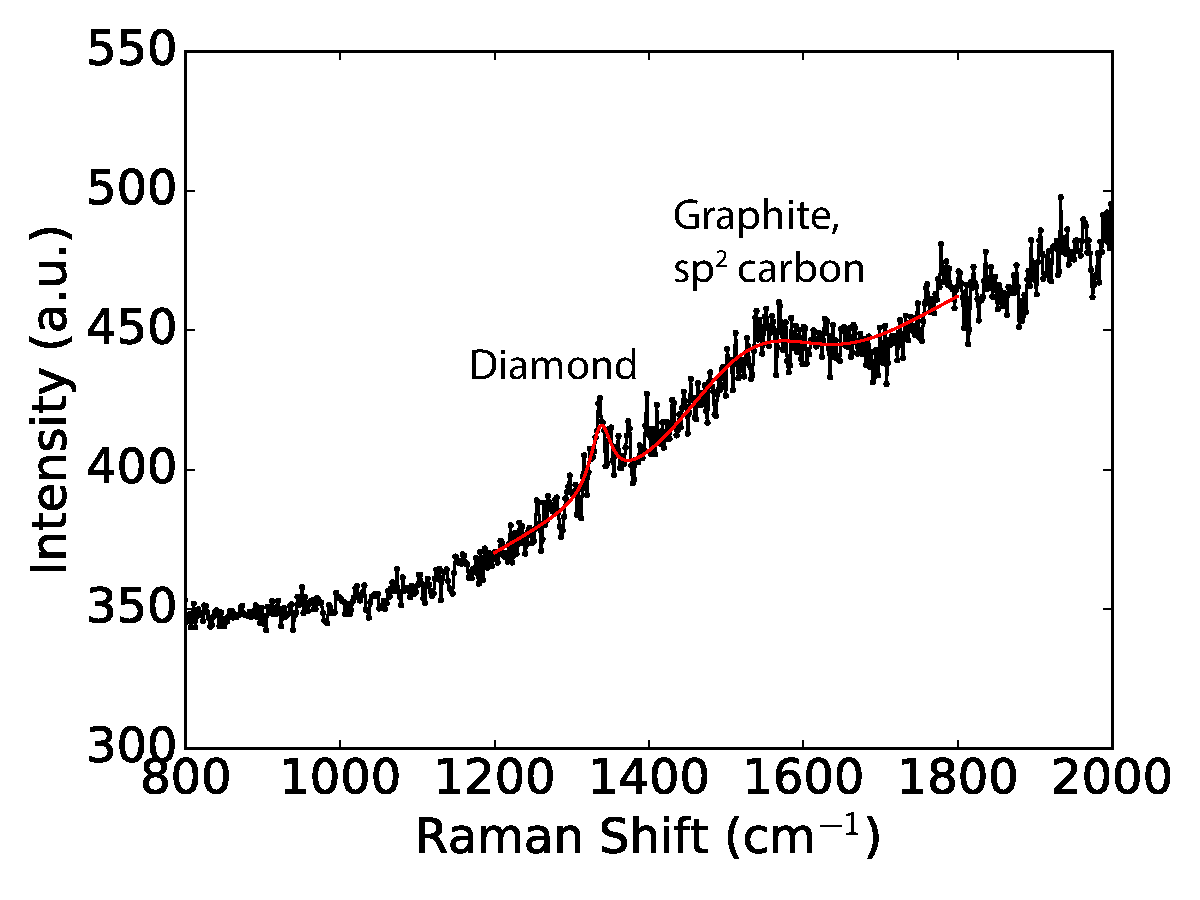
\includegraphics[trim = 0 0 0 0 , clip = true, width = \linewidth]{./pics/Ir25_spectrum_scan_xy-05x6y8_4000uW_t60_wavenumber_fit.pdf}}
			\end{subfigure}
			\hfill
			\begin{subfigure}[tp]{0.45\linewidth}
				\caption{}\label{subfig::raman_ox}
				\centering
				\testbox{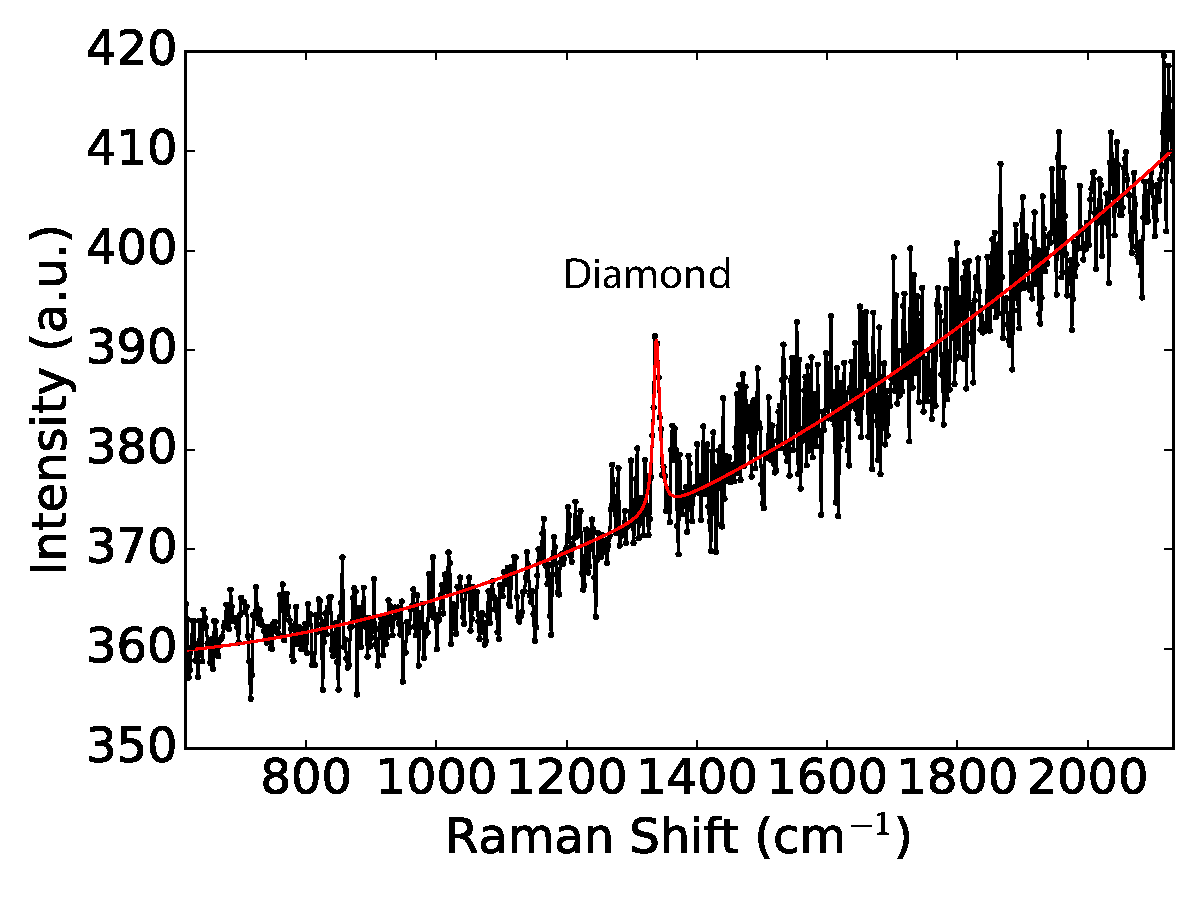
\includegraphics[trim = 0 0 0 0,  clip = true, width = \linewidth]{./pics/Ir_22_spe_scan_xy-02x7y7_550-600nm_t240_wavenumber_fit.pdf}}
			\end{subfigure}
			\caption{Raman measurements, black: data, red: fit. (a) Raman measurement before oxidation, sample \insituS. The diamond Raman peak is situated at \SI{1338}{\per\centi\meter}. The broad feature around \SI{1600}{\per\centi\meter} corresponds to the graphite G-band. (b) Raman measurement after oxidation, sample \insituSo. The G-band has vanished, indicating removal of graphite and amorphous sp$^2$ hybridized carbon.}
			\label{fig::raman}
		\end{figure}

		Raman measurements of the wet-milled \nds give insight to the issues of surface contamination, defects in the diamond lattice and strain in the lattice:
		Surface contamination like graphite and amorphous sp$^2$ hybridized carbon atoms cause additional peaks in the Raman spectrum. 
		A high defect concentration may lead to both additional peaks, to a broadening of the first order Raman peak and a shift to smaller wavenumbers.
		Strain in the diamond broadens the first order Raman peak and causes a shift to higher wavenumbers \cite{Zaitsev2001,Prawer2004,Orwa2000}.
		\\
		For the Raman measurements the same layout of the setup described in \autoref{ch::confocal_setup} is used.
		As excitation lightsource, a \SI{532}{nm} continuous wave diode laser is used (IO \todo[fancyline]{type}).
		It provides single (frequency) mode laser light, which is a prerequisite for Raman investigations.
		The beamsplitter is a dichroic mirror (DRLP645), the laser light is additionally filtered out with a 532 Notch filter in the detection path in front of the single mode fiber instead of the otherwise used longpass filter.
		With these adaptions, the combination of the confocal unit and the spectrometer serve as a Raman spectrometer.
		As the diamond Raman line is very narrow (~xx\todo[fancyline]{check number}), the \SI[per-mode=symbol]{600}{\lines\per\mm} grating is used for a first overview; for more detailed measurements the \SI[per-mode=symbol]{1200}{\lines\per\mm} and \SI[per-mode=symbol]{1800}{\lines\per\mm} gratings are used.
		\\
		Due to the low signal from a single \nd, the Raman measurements are carried out at several areas on the sample \insituS which are densely covered with \nds, hence taking measurements of clusters of \nds.
		The narrow peak in \autoref{subfig::raman_no} corresponds to the first order diamond Raman peak.
		The Raman shift of \SI{1338}{\per\centi\meter} compared to the literature value of \SI{1332}{\per\centi\meter} of pristine diamond \cite{Zaitsev2001} indicates the presence of strain in the diamond particles.
		Furthermore, the investigated Raman spectra show a broad peak with a Raman shift of about \SI{1582}{\per\centi\meter} (\autoref{subfig::raman_no}).
		This shift corresponds to the G-band due to amorphous sp$^2$ hybridized carbon atoms and graphite.
		The exact G-band position and \lw is sensitive to parameters such as the clustering of the sp$^2$ phase, bond-length and bond-angle disorder, presence of sp$^2$ rings or chains, and the sp$^2$/sp$^3$ ratio \cite{Ferrari2004}.
		\\
		\Nd Raman spectra are considerably modified after \ox in air at \SI{450}{\degreeCelsius}.
		To verify this, we perform Raman measurements on three different spots on a non-oxidized sample (\insituS), and for comparison on three different spots on a sample produced in the same process which is additionally oxidized.
		While the G-band peak is present in every measurement performed on the sample which was not oxidized, it is not present in any of the measurements performed after \ox (\autoref{subfig::raman_ox}), indicating successful removal of sp$^2$ hybridized carbon and surface graphite.
		The position of the diamond Raman peak is the same oxidized (\insituSo) and non-oxidized (\insituSn) samples, indicating no effect on strain in the diamond.
		On the other hand, the width of the diamond Raman peak is between \SIlist{15; 30}{\per\centi\meter} without \ox treatment, but is only \SIrange{9}{11}{\per\centi\meter} after the \ox process.
		A possible reason for a change of the width is improved crystal quality.
		This effect is also subject in the following paragraphs and will be explained in more detail there.
		\\
		For comparison, measurements of the Raman line were also carried out on the implanted sample \implantedTao. 
		These diamond particles are big enough to perform measurements on single \nds.
		We found one diamond Raman line at \SI[separate-uncertainty]{1308+-5}{\per\centi\meter}, one at \SI[separate-uncertainty]{1345+-5}{\per\centi\meter} and one at \SI[separate-uncertainty]{1348+-5}{\per\centi\meter} (given uncertainties are governed by spectrometer resolution).
		We have to distinguish two cases, a shift of the first order Raman line to higher versus lower wavenumbers than the first order Raman line of \SI{1332}{\per\centi\meter} in pristine diamond.
		\\
		As mentioned before, a Raman shift of the first order Raman line to lower wavenumbers and a broadening of the Raman line indicates defects in the diamond lattice \cite{Prawer2004}.
		The Raman line at \SI[separate-uncertainty]{1308+-5}{\per\centi\meter} exhibits a broad \lw of \SI[separate-uncertainty]{25+-5}{\per\centi\meter}.
		Therefore both the position and the \lw of the Raman line indicate that there are many defects present in the diamond.
		\\
		The other case is a shift of the first order Raman line towards higher wavenumbers.
		The shift of the first order Raman line to higher wavenumbers is attributed to strain in the diamond lattice.
		While under hydrostatic pressure, the triply degenerate first order Raman peak remains degenerate, under uniaxial and more complex stress configurations (biaxial stress, shear stress etc.) mode splitting occurs \cite{Prawer2004}.
		As the measured peaks at wavenumbers higher than the wavenumber in pristine diamond are broad, we attribute these peaks to stress configurations other than hydrostatic stress, where the mode splitting manifests itself in a broadening of the peak due to limited spectrometer resolution.
		\\
		To summarize, there are two cases, one where the first order Raman line hints at many defects present in the diamond lattice and the other that leads to the assumption that the stress configuration in the diamonds are uniaxial or more complicated stress configurations.
		In \autoref{subsec::spectra} we will show that both of these assumptions fit nicely to the results from the measured \pl spectra. 

	\section[TEM]{Transmission Electron Spectroscopy Measurements}{\label{sec::tem}}

			
		\begin{figure}[tp]
			\begin{subfigure}[t]{ 0.49\linewidth}
				\centering	
				\caption{}
				\testbox{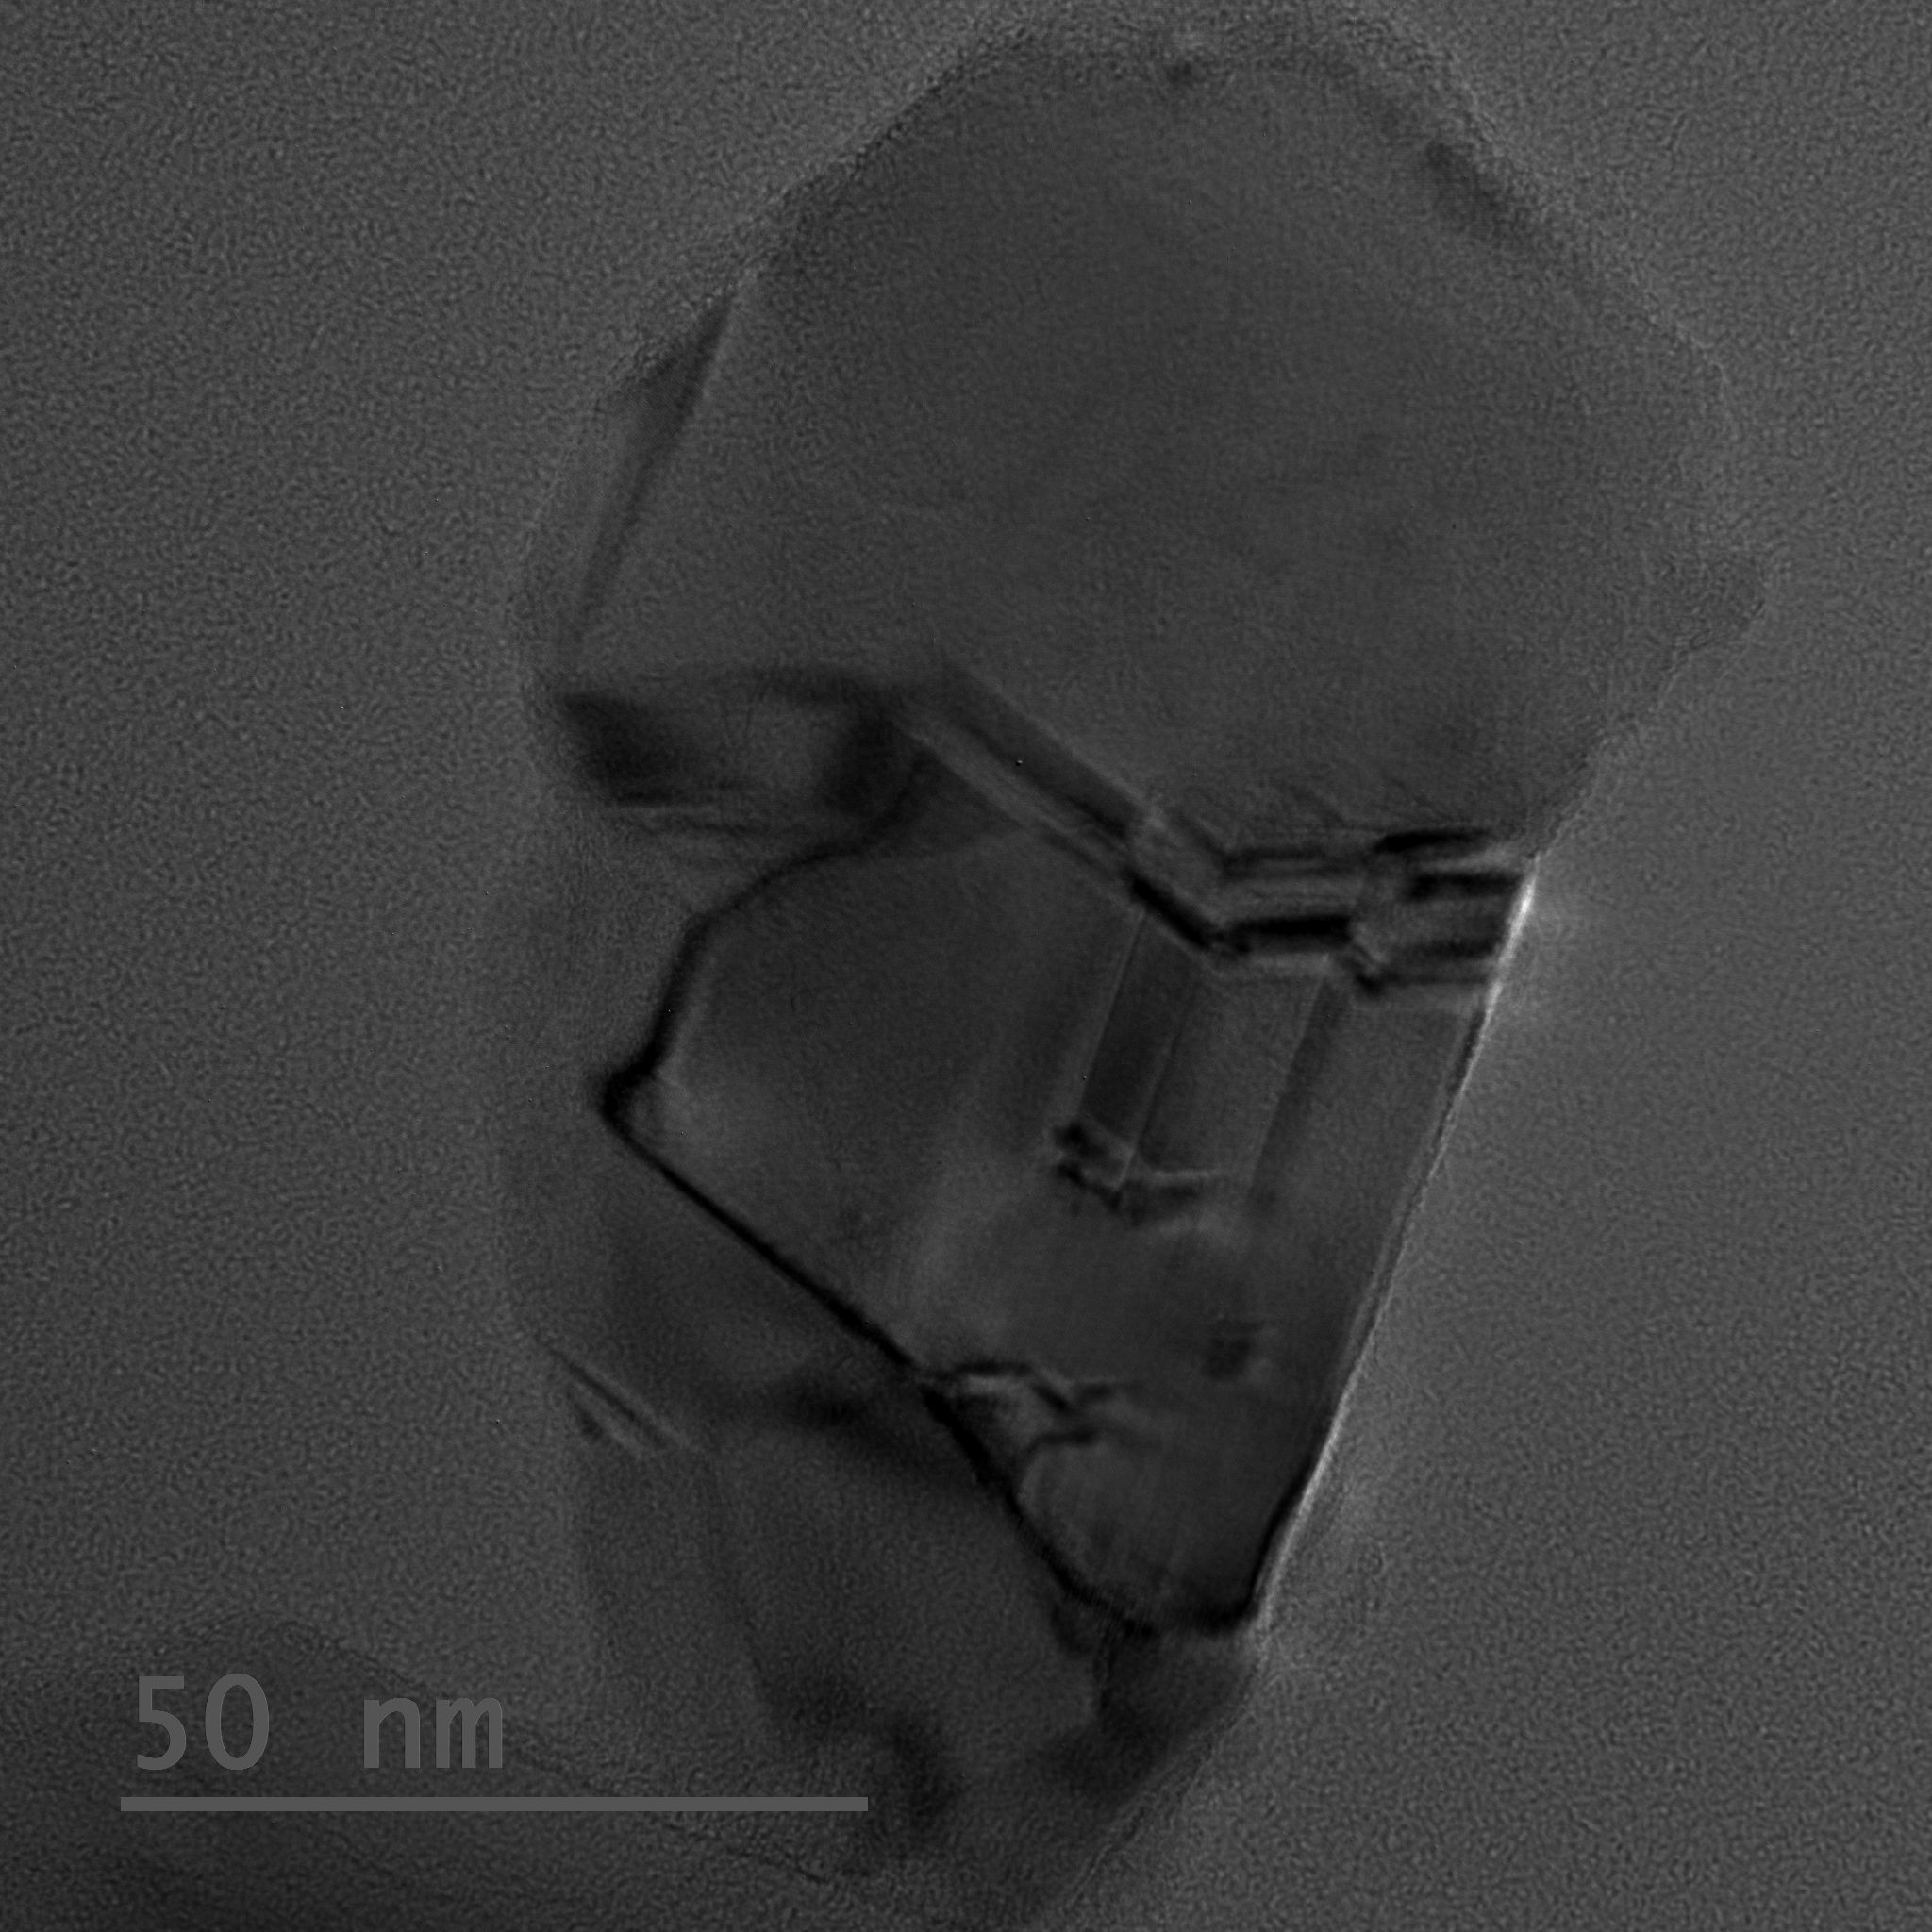
\includegraphics[trim = 0 0 0 0,  clip= true, width = \textwidth]{./pics/AM060-II-k4-2.png}}
				\label{subfig::tem_crystal}
			\end{subfigure}
			\hfill
			\begin{subfigure}[t]{ 0.49\linewidth}
				\centering
				\caption{}
				\testbox{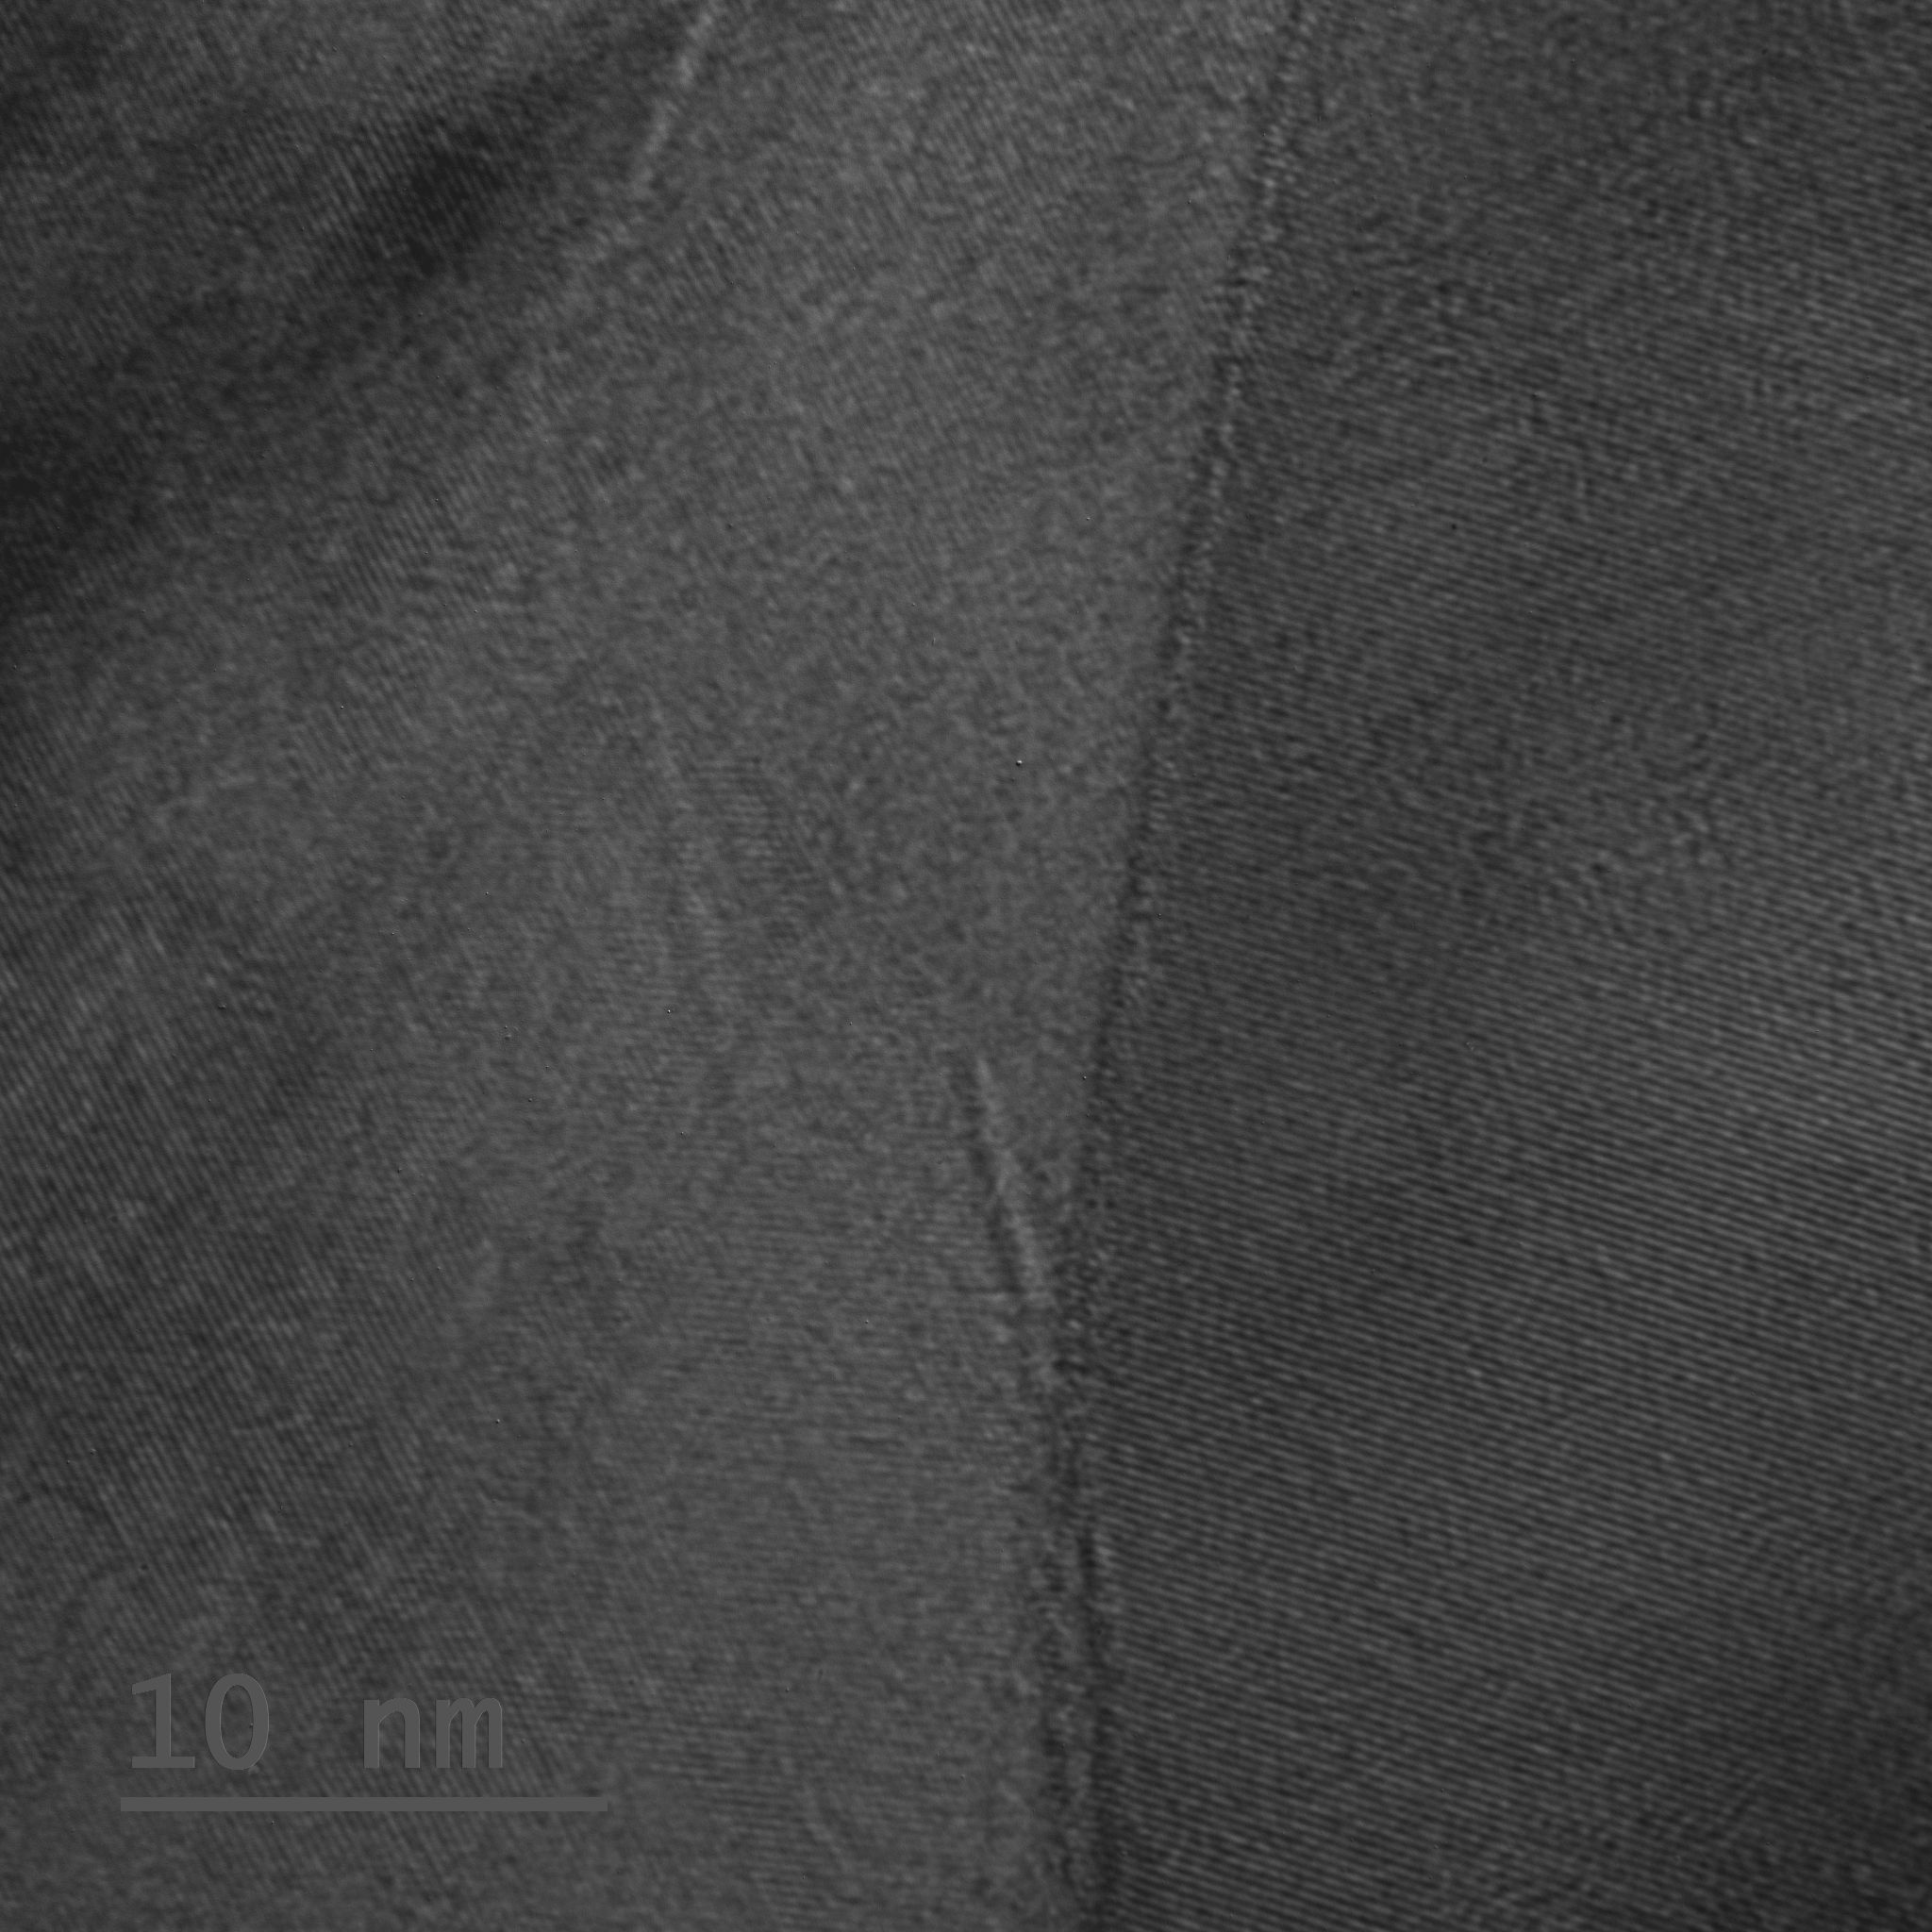
\includegraphics[trim = 0 0 0 0,  clip= true, width = \textwidth]{./pics/AM060-II-k1-3.png}}
				\label{subfig::tem_boundary}
			\end{subfigure}
			\caption{Transmission electron microscopy (TEM) pictures of sample \insituH. (a) Image of a single \nd particle. Several crystal boundaries can be seen within the diamond particle. (b) Close-up image a diamond particle. The vertical line is a crystal boundary, to the left and right the more or less horizontal layers of one crystalline region can be seen.}
			\label{fig::tem}
		\end{figure}


		\todo{beginning new text}We performed \tem (\TEM) measurements to further investigate the crystal quality\footnote{TEM measurements performed by \schmauch}.
		For those \TEM measurements, we used the sample \insituH.
		Smaller \nds would have been too small for the carbon grid which severs as a sample holder in the \TEM, and might have fallen through the grid and bigger bigger particles would have been too big to be transmitted by the electron beam, making the imaging impossible.
		In \autoref{fig::tem} there are \TEM images, one of them exhibits a single diamond particle and the other is a close-up image of a crystal boundary. 
		From \autoref{subfig::tem_crystal} it can be seen that the diamond particle contains several crystallites surrounded by crystal boundaries. 
		The crystal boundaries are the sharp features within the diamond particle.
		In \autoref{subfig::tem_boundary} the crystal layers which are more or less horizontal and in more or less the middle of the picture there is a vertical line which is a crystal boundary.
		So it is clear that the investigated sample does not contain beautiful single crystal diamond particles, which means a reduction of the crystal quality of the diamond particles.\todo{end new text}


